% !TeX root = ../thuthesis-example.tex

\chapter{燃面变化规律}
\section{图像绘制}

根据七组装药数据,在内弹道计算程序中进行计算,每组数据计算有无侵蚀两组,共获得14组燃面随时间变化数据。我们想要求出燃烧面积随肉厚的变化,下图绘制出了7组药柱$A_{b}$燃面随层厚$e$的变化规律。

\begin{figure}
  \centering
  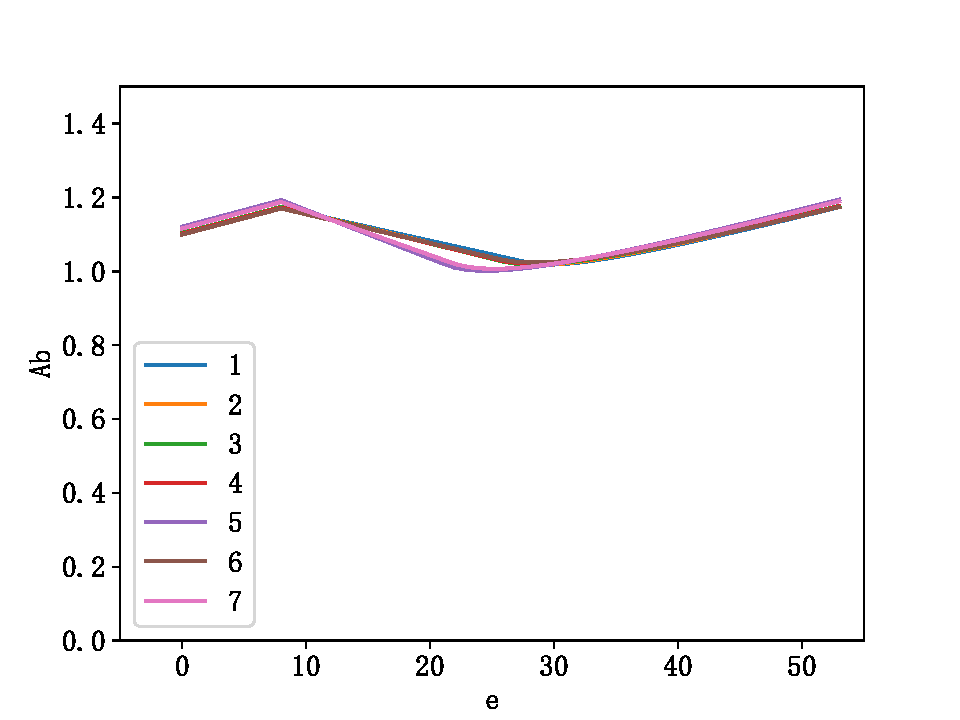
\includegraphics[width=0.7\linewidth]{燃面变化规律图.pdf}

  \caption{7组药柱燃面变化图}
  \label{fig:example}
\end{figure}

将曲线放大
\begin{figure}
    \centering
    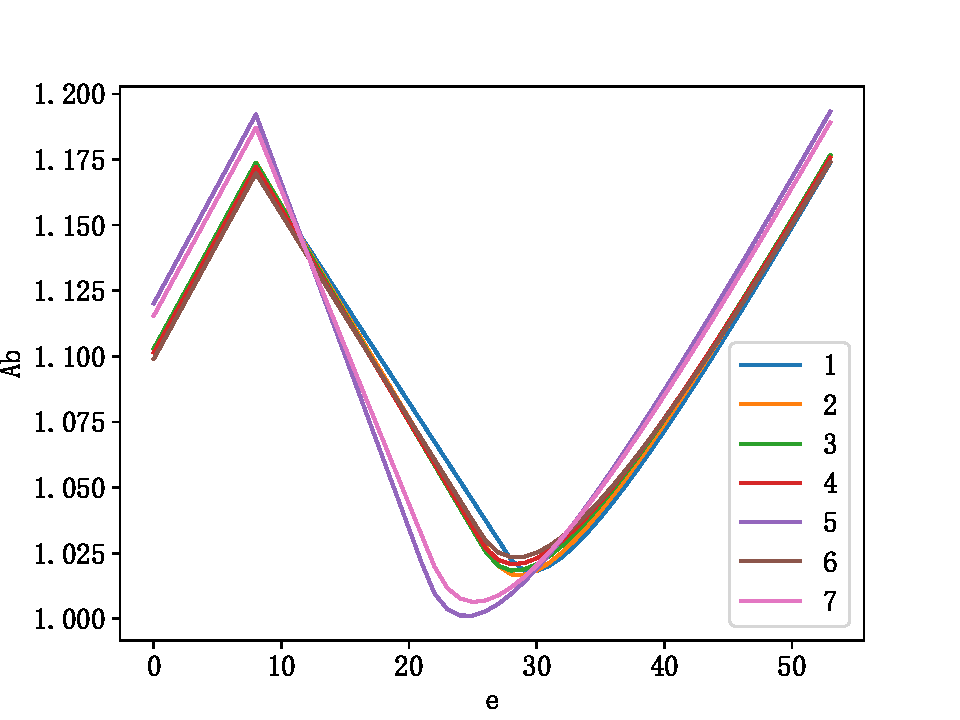
\includegraphics[width=0.7\linewidth]{燃面变化规律放大图.pdf}

    \caption{7组药柱燃面变化放大图}
    \label{fig:example}
  \end{figure}

\section{分析}
燃面变化分为上升、下降、上升三个阶段,第一段因为星角圆弧半径
引起的初始增面燃烧,第二段是由于$\theta < \overline{\theta }$而导致的减面燃烧,第三段因为星角消失导致的增面燃烧,所选药柱理论结果满足设计要求。

各曲线之间相差不大,最大值、最小值、转折点近似。同时,1、2、3、4、6号最大燃面与最小燃面大致相差0.125$m^2$,5、7号最大燃面与最小燃面大致相差0.18$m^2$,差值较小,接近于恒面燃烧的燃面变化规律。

5号药柱压力最大值和最小值的差值最大,5号组药柱达到压力最小值。

1、2、3、4、6号最大值和最小值的差值小,由侵蚀效应带来的效果最为明显。

1、2、3、4、6号重合度高,5、7号重合度高。

各组药柱第一阶段基本一致,第二阶段5、7号柱减面速率更快,之后第三阶段各药柱又一次基本一致。

5号药柱和第7号药柱初始燃面较大,侵蚀效应会比其他几组大。

6号装药燃烧面积波动最小,是7组合格药中恒面性最好的,即推力性能最平稳。